%% generato automaticamente da tools/build_tex.py --- non modificare
\chapter{Equazioni algebriche spezzate in due}
\label{cap:equazioni}
\quaderno{equazioni.dfw}{27 Jan 2010}{44}

Gennaio 2010. Il quaderno applica una sola idea a quattro casi, di grado crescente dal primo al quarto. L'idea è questa: invece di risolvere un'equazione algebrica nel campo complesso, si scrive l'incognita come $z=x+\mathrm{i}y$ con $x$ e $y$ reali, si separano parte reale e parte immaginaria, e si ottiene un sistema di due equazioni reali in due incognite. È il metodo che, in geometria, corrisponde a cercare le radici come intersezioni di due curve nel piano.

\section{Primo grado}

Il caso più semplice serve a fissare la procedura. Il risultato è noto, ma il modo in cui si arriva merita di essere visto perché è quello che verrà ripetuto tre volte.

\begin{espr}{1}{User}{}
\[
a\, z + b = 0
\]
\end{espr}
L'equazione di primo grado nel campo complesso.

\begin{espr}{2}{User}{}
\[
z = x + \mathrm{i}\, y
\]
\end{espr}
La sostituzione che genera tutto il resto.

\begin{espr}{3}{Sub(\#1)}{}
\[
a\, \left(x + \mathrm{i}\, y\right) + b = 0
\]
\end{espr}
Sostituita.

\begin{espr}{4}{User}{}
\[
a\, x + b + \mathrm{i}\, a\, y = 0
\]
\end{espr}
Sviluppata, con parte reale e immaginaria separate.

\begin{espr}{5}{User}{}
\[
\operatorname{Re}\!\left(a\, x + b + \mathrm{i}\, a\, y\right) = 0
\]
\end{espr}
La condizione sulla parte reale.

\begin{espr}{6}{User}{}
\[
\operatorname{Im}\!\left(a\, x + b + \mathrm{i}\, a\, y\right) = 0
\]
\end{espr}
E quella sulla parte immaginaria.

\begin{espr}{7}{User}{}
\[
z = -\frac{b}{a} + \mathrm{i}\, 0
\]
\end{espr}
La soluzione, scritta con la parte immaginaria esplicitamente nulla.


La parte immaginaria dà $ay=0$, cioè $y=0$: l'equazione di primo grado a coefficienti reali non ha radici fuori dall'asse reale. La parte reale dà allora $x=-b/a$. La riga $\#7$ scrive la soluzione nella forma completa $z=-b/a+\mathrm{i}\cdot0$, che sembra pedante ma è il punto: il metodo restituisce sempre una coppia, ed è la coppia a dire dove si trova la radice.

\section{Secondo grado}

Qui il metodo comincia a dare qualcosa in cambio. Sostituendo $z=x+\mathrm{i}y$ nella forma generale e separando, si ottengono due coniche.

\begin{espr}{8}{User}{}
\[
a\, z^{2} + b\, z + c = 0
\]
\end{espr}
L'equazione di secondo grado.

\begin{espr}{9}{User}{}
\[
z = x + \mathrm{i}\, y
\]
\end{espr}
La stessa sostituzione.

\begin{espr}{10}{User}{}
\[
a\, x^{2} + b\, x - a\, y^{2} + c + \mathrm{i}\, \left(2\, a\, x\, y + b\, y\right) = 0
\]
\end{espr}
Lo sviluppo. La parte immaginaria è già raccolta a fattor comune per $y$.

\begin{espr}{11}{User}{}
\[
\operatorname{Re}\!\left(a\, x^{2} + b\, x - a\, y^{2} + c + \mathrm{i}\, \left(2\, a\, x\, y + b\, y\right)\right) = 0
\]
\end{espr}
La condizione sulla parte reale: un'iperbole equilatera nel piano $(x,y)$.

\begin{espr}{12}{User}{}
\[
\operatorname{Im}\!\left(a\, x^{2} + b\, x - a\, y^{2} + c + \mathrm{i}\, \left(2\, a\, x\, y + b\, y\right)\right) = 0
\]
\end{espr}
La condizione sulla parte immaginaria.

\begin{espr}{13}{Simp(\#11)}{}
\[
a\, x^{2} + b\, x - a\, y^{2} + c = 0
\]
\end{espr}
Semplificata.

\begin{espr}{14}{Simp(\#12)}{}
\[
2\, a\, x\, y + b\, y = 0
\]
\end{espr}
Semplificata: il prodotto $y(2ax+b)$ deve annullarsi.

\begin{espr}{15}{Simp(User)}{}
\[
\left[\, x = -\frac{b}{2\, a} \;\land\; y = \frac{\sqrt{4\, a\, c - b^{2}}}{2\, \left|a\right|},\; x = -\frac{b}{2\, a} \;\land\; y = -\frac{\sqrt{4\, a\, c - b^{2}}}{2\, \left|a\right|},\; x = -\frac{\sqrt{b^{2} - 4\, a\, c} + b}{2\, a} \;\land\; y = 0,\; x = \frac{\sqrt{b^{2} - 4\, a\, c} - b}{2\, a} \;\land\; y = 0 \,\right]
\]
\end{espr}
I quattro casi. I primi due sono la coppia coniugata quando $4ac>b^2$, gli altri due le radici reali quando $b^2>4ac$.

\begin{figure}[htbp]
  \centering
  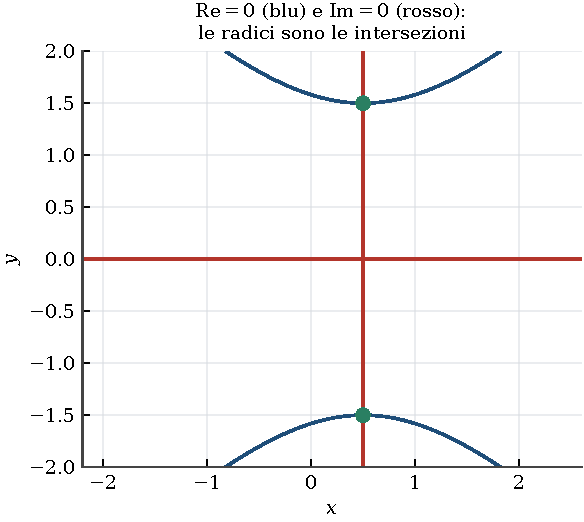
\includegraphics[width=0.62\linewidth]{../figures/equazioni_reim.pdf}
  \caption{Il metodo in figura, per $z^2-z+2{,}5=0$. La curva blu è il luogo $\operatorname{Re}=0$, la rossa il luogo $\operatorname{Im}=0$; quest'ultima è l'unione dell'asse reale e della verticale $x=-b/(2a)$, come impone la fattorizzazione. Le radici sono le intersezioni.}
  \label{fig:equazioni_reim}
\end{figure}

La parte immaginaria è $y(2ax+b)=0$, e questa fattorizzazione è tutto. O si annulla $y$ — e allora la radice è reale — oppure si annulla il secondo fattore, e allora $x=-b/(2a)$: le radici complesse stanno necessariamente sulla verticale per il vertice della parabola.

La riga $\#15$ elenca i quattro casi che ne derivano, e sono esattamente i due regimi della formula risolutiva. Se $4ac>b^2$ si hanno due radici coniugate con $x=-b/(2a)$ e $y=\pm\sqrt{4ac-b^2}/(2|a|)$; se $b^2>4ac$ si hanno due radici reali con $y=0$. Il discriminante non compare mai come tale: emerge da solo come condizione di realtà di una radice quadrata.

\section{Terzo grado}

Il grado tre è dove il metodo mostra la sua natura geometrica. La parte immaginaria continua a fattorizzarsi con $y$ in evidenza, ma il secondo fattore è ora una conica in $x$ e $y$.

\begin{espr}{16}{User}{}
\[
a\, z^{3} + b\, z^{2} + c\, z + d = 0
\]
\end{espr}
Si passa al terzo grado.

\begin{espr}{17}{User}{}
\[
z = x + \mathrm{i}\, y
\]
\end{espr}
Sostituzione.

\begin{espr}{18}{Sub(\#16)}{}
\[
a\, \left(x + \mathrm{i}\, y\right)^{3} + b\, \left(x + \mathrm{i}\, y\right)^{2} + c\, \left(x + \mathrm{i}\, y\right) + d = 0
\]
\end{espr}
Sostituita, senza sviluppare.

\begin{espr}{19}{User}{}
\begin{align*}
& a\, x^{3} + b\, x^{2} + x\, \left(c - 3\, a\, y^{2}\right) - b\, y^{2} + d + \mathrm{i}\, y\, \left(3\, a\, x^{2} + 2\, b\, x - a\, y^{2} + c\right) \\
=\;& 0
\end{align*}
\end{espr}
Sviluppata: la parte immaginaria è ancora un multiplo di $y$.

\begin{espr}{20}{User}{}
\begin{align*}
& \operatorname{Re}\!\left(a\, x^{3} + b\, x^{2} + x\, \left(c - 3\, a\, y^{2}\right) - b\, y^{2} + d + \mathrm{i}\, y\, \left(3\, a\, x^{2} + 2\, b\, x - a\, y^{2} + c\right)\right) \\
=\;& 0
\end{align*}
\end{espr}
Condizione sulla parte reale.

\begin{espr}{21}{User}{}
\begin{align*}
& \operatorname{Im}\!\left(a\, x^{3} + b\, x^{2} + x\, \left(c - 3\, a\, y^{2}\right) - b\, y^{2} + d + \mathrm{i}\, y\, \left(3\, a\, x^{2} + 2\, b\, x - a\, y^{2} + c\right)\right) \\
=\;& 0
\end{align*}
\end{espr}
E sulla parte immaginaria.

\begin{espr}{22}{Simp(\#20)}{}
\[
a\, x^{3} + b\, x^{2} + x\, \left(c - 3\, a\, y^{2}\right) - b\, y^{2} + d = 0
\]
\end{espr}
La cubica in $x$ con i termini in $y^2$.

\begin{espr}{23}{Simp(\#21)}{}
\[
y\, \left(3\, a\, x^{2} + 2\, b\, x - a\, y^{2} + c\right) = 0
\]
\end{espr}
Il prodotto che deve annullarsi. Il secondo fattore contiene la derivata della cubica.

\begin{espr}{24}{User}{}
\[
3\, a\, x^{2} + 2\, b\, x - a\, y^{2} + c = 0
\]
\end{espr}
Il secondo fattore isolato: una conica.

\begin{espr}{25}{Simp(Solve(\#24,y))}{}
\[
y = -\sqrt{\frac{3\, a\, x^{2} + 2\, b\, x + c}{a}} \;\lor\; y = \sqrt{\frac{3\, a\, x^{2} + 2\, b\, x + c}{a}}
\]
\end{espr}
Risolta rispetto a $y$: due rami simmetrici.

\begin{espr}{26}{User}{}
\[
y = 0
\]
\end{espr}
L'altro ramo della dicotomia.

\begin{espr}{27}{Sub(\#22)}{}
\begin{align*}
& a\, x^{3} + b\, x^{2} + x\, \left(c - 3\, a\, \left(-\sqrt{\frac{3\, a\, x^{2} + 2\, b\, x + c}{a}}\right)^{2}\right) - b\, \left(-\sqrt{\frac{3\, a\, x^{2} + 2\, b\, x + c}{a}}\right)^{2} \\
&\qquad + d \\
=\;& 0
\end{align*}
\end{espr}
Si sostituisce il valore di $y$ nella parte reale.

\begin{espr}{28}{Simp(\#27)}{}
\[
-\frac{8\, a^{2}\, x^{3} + 8\, a\, b\, x^{2} + 2\, x\, \left(a\, c + b^{2}\right) - a\, d + b\, c}{a} = 0
\]
\end{espr}
Il risultato: una cubica nella sola $x$, che dà l'ascissa della coppia coniugata.

\begin{espr}{29}{Simp(Solve(\#28,x))}{}
\begin{align*}
& x = \frac{-\sqrt{b^{2} - 3\, a\, c}\, \cos\!\left(\frac{\arccos\!\left(\frac{-\left(27\, a^{2}\, d - 9\, a\, b\, c + 2\, b^{3}\right)\, \operatorname{sgn}\!\left(a\right)}{2\, \left(b^{2} - 3\, a\, c\right)^{\frac{3}{2}}}\right)}{3}\right)}{3\, \left|a\right|} - \frac{b}{3\, a} \\[3pt]
\lor\quad & x = \frac{\sqrt{b^{2} - 3\, a\, c}\, \sin\!\left(\frac{\arcsin\!\left(\frac{\left(27\, a^{2}\, d - 9\, a\, b\, c + 2\, b^{3}\right)\, \operatorname{sgn}\!\left(a\right)}{2\, \left(b^{2} - 3\, a\, c\right)^{\frac{3}{2}}}\right)}{3} + \frac{\pi}{3}\right)}{3\, \left|a\right|} - \frac{b}{3\, a} \\[3pt]
\lor\quad & x = \frac{-\sqrt{b^{2} - 3\, a\, c}\, \sin\!\left(\frac{\arcsin\!\left(\frac{\left(27\, a^{2}\, d - 9\, a\, b\, c + 2\, b^{3}\right)\, \operatorname{sgn}\!\left(a\right)}{2\, \left(b^{2} - 3\, a\, c\right)^{\frac{3}{2}}}\right)}{3}\right)}{3\, \left|a\right|} - \frac{b}{3\, a}
\end{align*}
\end{espr}
\begin{espr}{30}{User}{}
\[
y = -\sqrt{\frac{3\, a\, x^{2} + 2\, b\, x + c}{a}} \;\lor\; y = \sqrt{\frac{3\, a\, x^{2} + 2\, b\, x + c}{a}}
\]
\end{espr}
I due rami, riscritti.

\begin{espr}{31}{Simp(Sub(\#22))}{}
\[
a\, x^{3} + b\, x^{2} + c\, x + d = 0
\]
\end{espr}
Sostituendo invece $y=0$ si ritrova l'equazione di partenza: il ramo delle radici reali.

\begin{espr}{32}{Simp(Solve(\#31,x))}{}
\begin{align*}
& x = \frac{2\, \sqrt{b^{2} - 3\, a\, c}\, \cos\!\left(\frac{\arccos\!\left(\frac{-\left(27\, a^{2}\, d - 9\, a\, b\, c + 2\, b^{3}\right)\, \operatorname{sgn}\!\left(a\right)}{2\, \left(b^{2} - 3\, a\, c\right)^{\frac{3}{2}}}\right)}{3}\right)}{3\, \left|a\right|} - \frac{b}{3\, a} \\[3pt]
\lor\quad & x = \frac{-2\, \sqrt{b^{2} - 3\, a\, c}\, \sin\!\left(\frac{\arcsin\!\left(\frac{\left(27\, a^{2}\, d - 9\, a\, b\, c + 2\, b^{3}\right)\, \operatorname{sgn}\!\left(a\right)}{2\, \left(b^{2} - 3\, a\, c\right)^{\frac{3}{2}}}\right)}{3} + \frac{\pi}{3}\right)}{3\, \left|a\right|} - \frac{b}{3\, a} \\[3pt]
\lor\quad & x = \frac{2\, \sqrt{b^{2} - 3\, a\, c}\, \sin\!\left(\frac{\arcsin\!\left(\frac{\left(27\, a^{2}\, d - 9\, a\, b\, c + 2\, b^{3}\right)\, \operatorname{sgn}\!\left(a\right)}{2\, \left(b^{2} - 3\, a\, c\right)^{\frac{3}{2}}}\right)}{3}\right)}{3\, \left|a\right|} - \frac{b}{3\, a}
\end{align*}
\end{espr}
\begin{espr}{33}{User}{}
\[
y = 0
\]
\end{espr}
Il ramo reale, esplicitato.


La dicotomia è la stessa di prima: $y=0$ oppure $3ax^2+2bx-ay^2+c=0$. Quest'ultima è un'iperbole (per $a>0$), e la riga $\#25$ ne ricava $y$ in funzione di $x$. Sostituendo nella parte reale si ottiene la riga $\#28$, una cubica in $x$ sola, che individua l'ascissa comune alla coppia di radici coniugate. La riga $\#31$ conferma il ramo reale: ponendo $y=0$ la parte reale ridiventa l'equazione di partenza.

Si noti che l'equazione $\#24$ contiene il polinomio $3ax^2+2bx+c$, cioè la derivata della cubica: le radici complesse di un polinomio di terzo grado si trovano sopra e sotto il punto in cui la derivata compensa il termine $ay^2$. È una relazione fra il polinomio e la sua derivata che il metodo produce senza che nessuno l'abbia cercata.

\section{Quarto grado}

L'ultimo caso ripete lo schema una volta di più, ed è quello che chiarisce che si tratta di un fenomeno generale.

\begin{espr}{34}{User}{}
\[
a\, x^{4} + b\, x^{3} + c\, x^{2} + d\, x + e = 0
\]
\end{espr}
Si passa al quarto grado.

\begin{espr}{35}{User}{}
\[
z = x + \mathrm{i}\, y
\]
\end{espr}
Sostituzione.

\begin{espr}{36}{Sub(\#34)}{}
\begin{align*}
& a\, \left(x + \mathrm{i}\, y\right)^{4} + b\, \left(x + \mathrm{i}\, y\right)^{3} + c\, \left(x + \mathrm{i}\, y\right)^{2} + d\, \left(x + \mathrm{i}\, y\right) \\
&\qquad + e \\
=\;& 0
\end{align*}
\end{espr}
Sostituita.

\begin{espr}{37}{User}{}
\begin{align*}
& a\, x^{4} + b\, x^{3} + x^{2}\, \left(c - 6\, a\, y^{2}\right) + x\, \left(d - 3\, b\, y^{2}\right) + a\, y^{4} - c\, y^{2} + e + \mathrm{i}\, y\, \left(4\, a\, x^{3} + 3\, b\, x^{2} + 2\, x\, \left(c - 2\, a\, y^{2}\right) - b\, y^{2} + d\right) \\
=\;& 0
\end{align*}
\end{espr}
Sviluppata.

\begin{espr}{38}{User}{}
\begin{align*}
& \operatorname{Re}\!\left(a\, x^{4} + b\, x^{3} + x^{2}\, \left(c - 6\, a\, y^{2}\right) + x\, \left(d - 3\, b\, y^{2}\right) + a\, y^{4} - c\, y^{2} + e + \mathrm{i}\, y\, \left(4\, a\, x^{3} + 3\, b\, x^{2} + 2\, x\, \left(c - 2\, a\, y^{2}\right) - b\, y^{2} + d\right)\right) \\
=\;& 0
\end{align*}
\end{espr}
Condizione sulla parte reale.

\begin{espr}{39}{Simp(\#38)}{}
\[
a\, x^{4} + b\, x^{3} + x^{2}\, \left(c - 6\, a\, y^{2}\right) + x\, \left(d - 3\, b\, y^{2}\right) + a\, y^{4} - c\, y^{2} + e = 0
\]
\end{espr}
Semplificata: una quartica in $x$ con termini in $y^2$ e $y^4$.

\begin{espr}{40}{User}{}
\begin{align*}
& \operatorname{Im}\!\left(a\, x^{4} + b\, x^{3} + x^{2}\, \left(c - 6\, a\, y^{2}\right) + x\, \left(d - 3\, b\, y^{2}\right) + a\, y^{4} - c\, y^{2} + e + \mathrm{i}\, y\, \left(4\, a\, x^{3} + 3\, b\, x^{2} + 2\, x\, \left(c - 2\, a\, y^{2}\right) - b\, y^{2} + d\right)\right) \\
=\;& 0
\end{align*}
\end{espr}
Condizione sulla parte immaginaria.

\begin{espr}{41}{Simp(\#40)}{}
\[
y\, \left(4\, a\, x^{3} + 3\, b\, x^{2} + 2\, x\, \left(c - 2\, a\, y^{2}\right) - b\, y^{2} + d\right) = 0
\]
\end{espr}
Ancora il fattore $y$, e ancora la derivata del polinomio nel secondo fattore.

\begin{espr}{42}{User}{}
\[
y = 0
\]
\end{espr}
Il ramo reale.

\begin{espr}{43}{Simp(Sub(\#39))}{}
\[
a\, x^{4} + b\, x^{3} + c\, x^{2} + d\, x + e = 0
\]
\end{espr}
Che restituisce la quartica di partenza.

\begin{espr}{44}{User}{}
\[
4\, a\, x^{3} + 3\, b\, x^{2} + 2\, x\, \left(c - 2\, a\, y^{2}\right) - b\, y^{2} + d = 0
\]
\end{espr}
Il secondo fattore isolato: la cubica che individua le coppie coniugate.


Ancora una volta la parte immaginaria si fattorizza come $y\cdot(\ldots)$, e il fattore fra parentesi contiene $4ax^3+3bx^2+2cx+d$ — di nuovo la derivata del polinomio di partenza, corretta da termini in $y^2$. La ragione è semplice e vale per ogni grado: se $p$ ha coefficienti reali, allora
\[
  \operatorname{Im} p(x+\mathrm{i}y)=y\,\big[p'(x)+O(y^2)\big],
\]
perché lo sviluppo di Taylor $p(x+\mathrm{i}y)=p(x)+\mathrm{i}yp'(x)-\tfrac{y^2}{2}p''(x)-\cdots$ ha parte immaginaria composta dai soli termini di grado dispari in $y$. Il fattore $y$ si raccoglie sempre, e il primo termine è sempre la derivata. Le quattro sezioni del quaderno sono quattro istanze di questa identità.

\section*{In sintesi}
\addcontentsline{toc}{section}{In sintesi}

Il metodo non è competitivo come strumento di calcolo — per risolvere un'equazione di secondo grado la formula è più rapida. Vale però come strumento di comprensione: rende visibile perché le radici complesse di un polinomio reale vengano a coppie, perché stiano su una verticale nel caso quadratico, e perché la derivata del polinomio compaia sempre nella condizione che le governa. Quattro gradi svolti per esteso sono più che sufficienti a mostrarlo.

